\chapter{Cuantificación de Cationes Metálicos}\label{sec:quantification}
\vspace{-1cm}%\enlargethispage{\baselineskip}
Para cuantificar los cationes metálicos se empleó un espectrómetro de absorción atómica Perkin-Elmer 3100 siguiendo las especificaciones recomendadas por el fabricante \citep{perkin}. El instrumento puede configurarse para trabajar en modo \ac{FAAS} y en modo \ac{FAES}. Las condiciones instrumentales empleadas para cada ele\-mento se encuentran en la Tabla~\ref{tab:FAASconditions}. En todos los casos se usó una llama oxidante (azul) de aire/acetileno en relación de volumen~2:1. 

\newcolumntype{P}[1]{>{\centering\arraybackslash}p{#1}}
\begin{table}[H]
    \centering\footnotesize
    \begin{tabular}{@{}p{1.5cm}P{1cm}P{2.6cm}P{1cm}P{1cm}P{1cm}l@{}}\toprule
        \multirow{2}{*}{\textbf{Elemento}}&$\lambda$ &\textbf{RT} &\textbf{AR} &\textbf{TI} &\textbf{ICL}&\textbf{Modelo}\\
        &(nm)&(mg~kg$^{-1}$)&(nm)&(s)&(mA)\\\midrule
        Litio   &670.8 &5 - 250 (\e{-3}) & 0.7& 0.3&(FAES) & Lineal\\
                &      &0.05 - 2.00 & 0.7& 0.5&8 & Lineal\\
        Sodio   &589.0 &0.10 - 8.00 & 0.4& 0.5&(FAES) & Cuadrático\\
        Potasio &776.5 &0.20 - 2.30 & 0.7& 0.5&(FAES) & Cuadrático\\
        Magnesio&285.2 &0.23 - 1.16 & 0.7& 0.5&verificar \\
        Calcio  &427.7 &1.00 - 5.15 & 0.7& 0.5&verificar \\\bottomrule
        \multicolumn{7}{@{}l@{}}{\tiny\textbf{RT:} Rango de trabajo; \textbf{AR:} Ancho de rendija; \textbf{TI:} Tiempo de integración; \textbf{ICL:} Intensidad de corriente de la lámpara}
    \end{tabular}
    \caption{Condiciones instrumentales para la determinación de elementos por FAAS y FAES.}
    \label{tab:FAASconditions}
\end{table}

\vspace{-0.7cm}En el presente trabajo fue necesario trabajar con muestras altamente salinas como agua de mar (más de 35~g~kg\mnn\ de sólidos disueltos). Estas muestras no podían ser diluidas para determinar la concentración del litio que se encuentra a un muy bajo nivel. Tras la lectura de tales disoluciones el efecto memoria del instrumento era evidente y recalcitrante. El amarillo color característico de la llama con sodio no desaparecía fácilmente si se esperaba a lavar la cámara de nebulización con protocolos normales como aspirar agua desionizada o ácido diluido por un par de minutos. Para minimizar el consumo de combustible y el tiempo requerido para eliminar el efecto memoria se propuso cerrar el flujo de acetileno y subir al máximo el flujo de aire mientras se aspira por el capilar una mezcla de ácido nítrico 2\% con ácido clorhídrico 3\% en agua desionizada. La mezcla de ácidos en combinación con el alto flujo de aire disminuyó considerablemente el tiempo requerido para limpiar la cámara y dejar el equipo listo para determinar el siguiente elemento.


\section{Determinación de litio}
La cuantificación de litio se abordó desde diversos enfoques dependiendo de las características del experimento realizado. Se usó curva de calibración por patrón externo con concordancia de matriz para experimentos en los que las matrices de las disoluciones de alimentación y de recuperación no variaron significativamente durante el proceso de transporte. Si durante el experimento una de las disoluciones varía sistemáticamente de manera medible en un solo parámetro que se conoce afecta la respuesta del método (e.g. aumento paulatino de iones sodio en la fase de recuperación), la técnica de cuantificación aplicada fue regresión plana. Finalmente, en experimentos que involucraron matrices complejas como agua de mar (sintética o natural), se cuantificó el litio haciendo uso de la adición estándar de un solo punto.

La disolución concentrada de litio que fue utilizada como patrón inicial fue preparada con carbonato de litio seco que se disolvió en un ligero exceso de ácido clorhídrico. Para la cuantificación por estándar externo con concordancia de matriz o con regresión multiparamétrica se utilizó \ac{FAAS} y para la cuantificación por adición estándar de un solo punto se utilizó \ac{FAES} que es más sensible a bajas concentraciones.

\subsection{Concordancia de matriz}\label{sec:liexternal}
Las curvas de calibración por \ac{FAAS} para litio en ácido clorhídrico 0.1~mol~kg\mnn\ (fase de recuperación) y en hidróxido de sodio 0.1~mol~kg\mnn\ (fase de alimentación) se muestran en la Figura \ref{fig:LitCurve}. Los estándares de calibración fueron preparados por dilución gravimétrica de la disolución concentrada.

\begin{figure}[H]
    \centering
    \subbottom{\begin{picture}(242,170)
               \put(0, 0){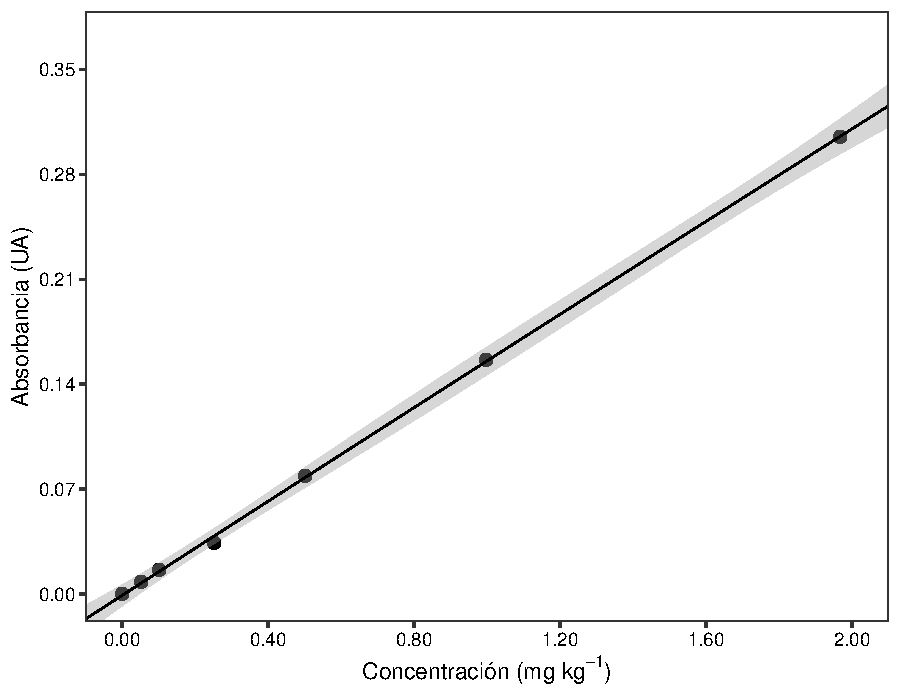
\includegraphics[height=0.388\textwidth]{App/images/LiCurves.pdf}}
               \put(24, 168){\large a)}
               \end{picture}}%
    \subbottom{\begin{picture}(230,170)
               \put(0, 0){\includegraphics[height=0.388\textwidth, trim={1.3cm 0 0 0}, clip, page=2]               {App/images/LiCurves.pdf}}
               \put(5, 168){\large b)}
               \end{picture}}\\
    \caption[Curvas de calibración para litio en medio ácido y en medio alcalino1.]{Curvas de calibración para litio en ácido clorhídrico 0.1~mol~kg\mnn\ (a) y en hidróxido de sodio 0.1~mol~kg\mnn\ (b) por FAAS. Se incluyen las curvas de regresión lineal donde la zona sombreada gris es el intervalo de confianza para la regresión con una significancia del 99\%.}
    \label{fig:LitCurve}
\end{figure}
\clearpage Las ecuaciones que describen las curvas de calibración para la fase de recuperación y de alimentación se muestran en las Ecuaciones \ref{eq:litRec} y \ref{eq:litAli}.
\begin{equation}\label{eq:litRec}
    Abs_{670.8~nm}=(0.000\pm0.001)+(0.156\pm0.002) C_{\ce{Li^+}}
\end{equation}
\begin{equation}\label{eq:litAli}
    Abs_{670.8~nm}=(0.000\pm0.001)+(0.183\pm0.002) C_{\ce{Li^+}}
\end{equation}
donde la concentración de litio ($C_{\ce{Li^+}}$) se encuentra en mg~kg\mnn. Hay diferencias estadísticamente significativas entre las pendientes de las curvas indicando que hay un efecto matriz presente que debe ser tenido en cuenta.


\subsection{Regresión multiparamétrica (plana)}\label{sec:planar1}
La presencia de iones sodio magnifica la señal de absorbancia de litio. Una regresión bivariada que considere la concentración de sodio entre las variables explicatorias puede mitigar el sesgo que se observa a causa de este factor. La regresión plana se hizo para considerar el efecto de cantidades variables de sodio que es transportado a la fase de recuperación durante el proceso de transporte. Un plano de regresión para valores de concentración de litio entre 0.05 y 2.00~mg~kg\mnn\ en presencia de cantidades variables de sodio (entre 0 y 250~mg~kg\mnn) se muestra en la Figura \ref{fig:planarLit}. Los estándares de calibración fueron preparados gravimétricamente a partir de la dilución de disoluciones concentradas de cloruro de litio y de sodio.

\begin{figure}[H]
    \centering
    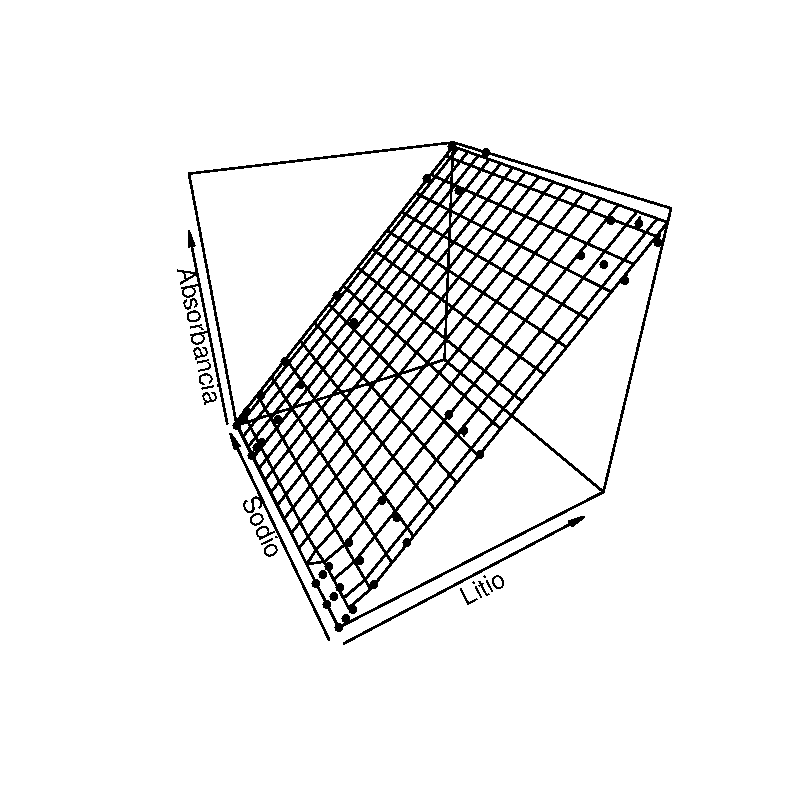
\includegraphics[width=0.5\textwidth, trim={3cm 2.5cm 2.05cm 2.3cm}, clip]{App/images/LiPlane.pdf}
    \caption{Plano de calibración para litio considerando la concentración de sodio.}
    \label{fig:planarLit}
\end{figure}
\clearpage La relación con el litio es similar a la presentada en las curvas de la Figura \ref{fig:LitCurve}. Puede observarse una inclinación ligera en el plano a medida que aumenta la concentración de sodio. La ecuación del plano es:
\begin{equation}\label{eq:litPlan}
    Abs_{670.8~nm}=(-0.002\pm0.001)+(0.1588\pm0.0008) C_{\ce{Li^+}}+(3.2\pm0.7)\e{-5} C_{\ce{Na^+}}
\end{equation}
donde la concentración de las especies está en mg~kg\mnn. 

El intercepto del plano sigue sin ser estadísticamente diferente de cero. La dependencia de la señal frente a la concentración de litio y de sodio sí es estadísticamente significativa. La sensibilidad del método hacia el litio es cuatro órdenes de magnitud mayor que hacia el sodio. Sin embargo, la concentración de sodio en la disolución de recuperación puede aumentar mucho más rápido que la del litio con lo que el efecto llegaría a ser importante y la regresión multiparamétrica podría ser de utilidad. Para calcular la concentración de litio a partir de una medición de absorbancia empleando el plano de regresión es necesario conocer (medir) la concentración de sodio en las disoluciones. 

\subsection{Adición estándar de un solo punto}
La disolución de recuperación sufre cambios drásticos cuando se extrae litio desde agua de mar sintética o natural. La mejor manera de contrarrestar el efecto matriz en la cuantificación de litio como consecuencia de estos cambios es por medio del método de adiciones estándar. La cuantificación de especies por adiciones estándar requiere que la señal del mesurando sea medida en conjunto con otras disoluciones enriquecidas con el mismo analito a determinar a un nivel conocido. La estrategia es eficiente para corregir los efectos matriz rotacionales cuyo efecto es un cambio en la sensibilidad del método (i.e.\ la pendiente de la curva de calibración) debido a la presencia de otros componentes.

Las adición estándar asume que una respuesta nula es producida por una muestra en la que la concentración de analito es también nula. La manera más común de obtener un resultado implica graficar la señal medida contra la concentración de analito adicionada. Debe incluirse el dato de la señal de la muestra sin enriquecer que corresponde a la señal de la muestra original. La extrapolación de los datos obtenidos hasta su intercepto con el eje de las abscisas corresponde al inverso aditivo de la concentración del analito en la muestra original.

Este método presenta la desventaja de que consume un mayor tiempo en la preparación de las muestras pues es equivalente a preparar una curva de calibración por cada muestra. Sin embargo, se ha demostrado que una cuantificación con buenas cualidades metrológicas puede obtenerse con la adición de un solo punto de muestra enriquecida \citep{Ellison2008}. Se recomienda que la muestra original y la muestra enriquecida sean diluidas de igual manera para que los constituyentes de la matriz original se encuentren a la misma concentración en ambas disoluciones. Sin embargo, cuando el factor de dilución que sufre la muestra enriquecida como consecuencia de la masa de disolución estándar adicionada es pequeño, este efecto es pequeño y puede ser despreciado.

En términos prácticos se divide la muestra disponible en dos viales, de los cuales en uno debe medirse la masa de disolución que ha sido agregada. El vial que contiene la masa conocida de disolución ($m_0$, cerca de 600~mg en nuestro caso) es adicionado con una masa conocida ($m_s$, cerca de 60~mg) de disolución estándar de litio con concentración conocida ($C_{\ce{Li+}}^{stock}$, 530~$\mu$g~kg\mnn). Se debe medir la señal de emisión de litio en la muestra original ($Em_{670.8~nm}^0$) y de la muestra enriquecida que debe ser cuidadosamente homogeneizada antes de la medición ($Em_{670.8~nm}^s$). La ecuación que se emplea en para conocer la concentración original de litio en la muestra ($C_{\ce{Li+}}^0$) es:
\begin{equation}
    C_{\ce{Li+}}^0 = C_{\ce{Li+}}^{stock} \cdot\frac{Em_{670.8~nm}^0  \big(\frac{m_s}{m_s+m_0}\big)} {Em_{670.8~nm}^s-Em_{670.8~nm}^0\big(\frac{m_0}{m_s+m_0}\big)}
\end{equation}
Es indispensable que ambas mediciones de emisión atómica caigan en el rango lineal del método. Para esto, el máximo de emisión en el instrumento se configuró con el estándar que es añadido para enriquecer las muestras ($\sim500~\mu$g~kg\mnn). Esto proporciona un excelente rango lineal entre 5 y 270~$\mu$g~kg\mnn\ como se muestra en la Figura \ref{fig:Rangolineal}. Ninguna muestra original o enriquecida debe tener una emisión mayor a la del límite superior del rango lineal y si esto se presenta, la muestra debe ser diluida gravimétricamente.

\begin{figure}[H]
    \centering
    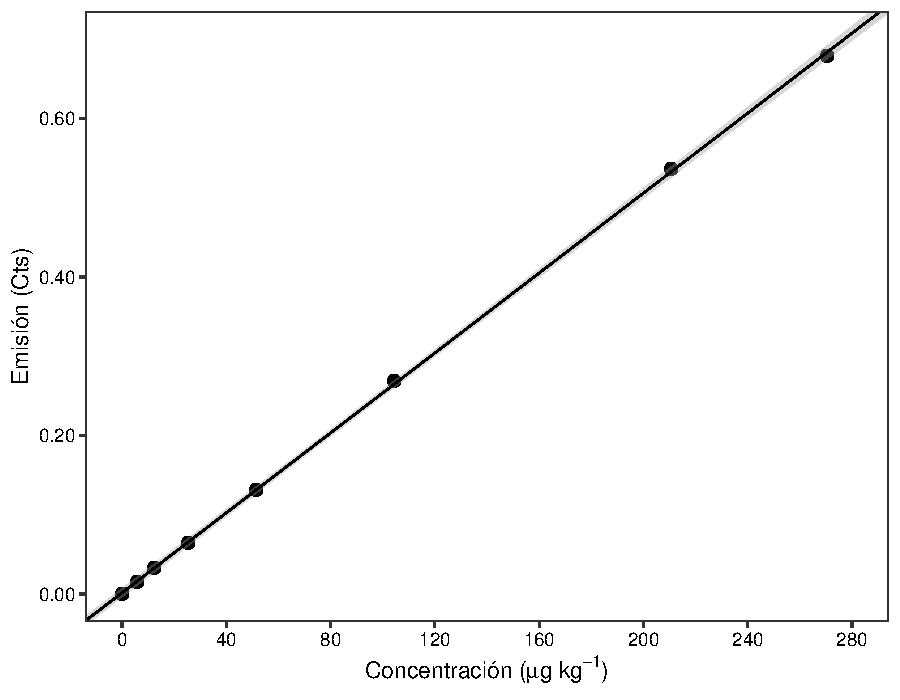
\includegraphics[height=0.388\textwidth]{App/images/LiRange.pdf}
    \caption[Rango lineal de la emisión de litio a bajas concentraciones]{Rango lineal de la emisión de litio a bajas concentraciones. Se incluye la curva de regresión lineal donde la zona sombreada gris es el intervalo de confianza para la regresión con una significancia del 99\%.}
    \label{fig:Rangolineal}
\end{figure}

\section{Determinación de sodio y potasio}
Las especies sodio y potasio fueron cuantificadas por \ac{FAES} usando curvas de calibración por patrón externo que se ajustaron a polinomios de grado 2. Los estándares de calibración se prepararon por dilución sucesiva de disoluciones concentradas de estos cationes que fueron preparadas a partir de sus respectivas sales de cloruro secas. Para disminuir el sesgo en las determinaciones, los estándares de calibración se prepararon en matrices similares a aquellas de las muestras considerando sus respectivos factores de dilución.

La baja energía de ionización de los metales alcalinos los hace susceptibles de perder electrones en el proceso de atomización y sus especies iónicas no presentan las mismas líneas de absorción o emisión de las especies atómicas. Esto ocasiona una disminución en la señal de estos elementos que se conoce como \textit{interferencia no espectral por ionización}. La mejor manera de corregir este tipo de interferencia es con la adición de un \textit{amortiguador de ionización} que es una especie fácilmente ionizable (generalmente metales alcalinos) que debe encontrarse a concentraciones altas. Los amortiguadores de ionización más utilizados son sales cloruro de potasio, cesio, litio y lantano a una concentración final en disolución de 0.1\%. 

Ejemplos de las curvas de calibración para sodio y potasio se muestran en la Figura \ref{fig:SodPot}. Las curvas fueron obtenidas usando cloruro de potasio para la determinación de sodio y cloruro de litio para la determinación de potasio (amortiguadores de ionización). En ambos casos se usó el estándar de más alta concentración para configurar el máximo de emisión respecto al cual son medidos los demás estándares y las muestras.

Las curvas obtenidas presentan un excelente ajuste y el intervalo de confianza a un nivel de significancia de 0.99 es muy delgado. Se probó el desempeño de los cloruros de lantano y de cesio como supresores de ionización pero dieron lugar a curvas de calibración con muy mala correlación por lo que no fueron incluidas. 

\begin{figure}[H]
    \centering
    \subbottom{\begin{picture}(242,170)
               \put(0, 0){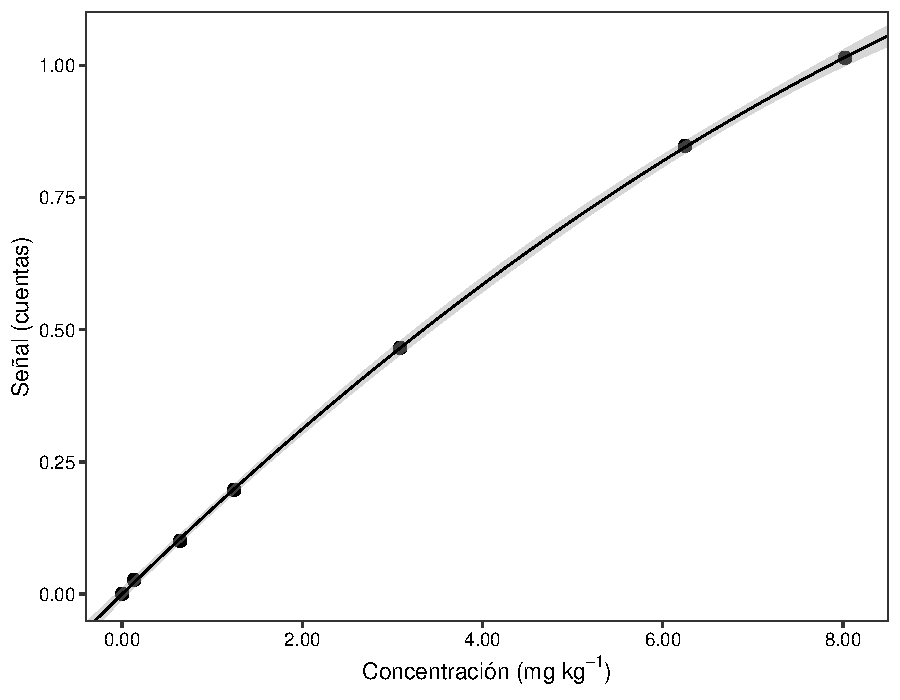
\includegraphics[height=0.388\textwidth]{App/images/NatKalCurves.pdf}}
               \put(24, 168){\large a)}
               \end{picture}}%
    \subbottom{\begin{picture}(230,170)
               \put(0, 0){\includegraphics[height=0.388\textwidth, trim={1.35cm 0 0 0}, clip, page=2]               {App/images/NatKalCurves.pdf}}
               \put(5, 168){\large b)}
               \end{picture}}\\
    \caption[Curvas de calibración para sodio y potasio por FAES.]{Curvas de calibración para sodio en cloruro de potasio 0.1\% (a) y potasio en cloruro de litio 0.1\% (b) por FAES. Se incluyen las curvas de regresión cuadrática donde la zona sombreada gris es el intervalo de confianza para la regresión con una significancia del 99\%.}
    \label{fig:SodPot}
\end{figure}

Las respectivas ecuaciones que describen las curvas de calibración se muestran en las Ecuaciones \ref{Eq:Nat} y \ref{Eq:Pot}. Los interceptos de las curvas con el eje de las ordenadas no son estadísticamente significativos.

\vspace{-0.8cm}
\begin{equation}\label{Eq:Nat}
    Em_{589.0~nm}=(0.000\pm0.002)+(0.166\pm0.002) C_{\ce{Na^+}} - (0.0049\pm0.0003) C_{\ce{Na^+}}^2
\end{equation}
\begin{equation}\label{Eq:Pot}
    Em_{776.5~nm}=(0.000\pm0.002)+(0.496\pm0.005) C_{\ce{K^+}} - (0.047\pm0.002) C_{\ce{K^+}}^2
\end{equation}
donde la concentración de las especies ($C_{\ce{M^+}}$) se encuentra en mg~kg\mnn. Los parámetros de las ecuaciones de regresión varían ligeramente en función de la temperatura de los estándares, la altura del quemador, el flujo del nebulizador y el instrumento que se utilice.

\section{Determinación de magnesio y calcio}
Las especies magnesio y calcio fueron cuantificadas por \ac{FAAS} usando curvas de calibración por patrón externo que presentaron un buen ajuste a una función cuadrática y lineal, respectivamente. Los estándares de calibración se prepararon por dilución sucesiva de di\-so\-luciones concentradas de estos cationes que fueron preparadas a partir de sus respectivas sales de carbonato secas disueltas en un ligero exceso de ácido clorhídrico.

Estas especies forman compuestos refractarios cuando hay fosfatos en el medio. La formación de estos compuestos refractarios impide la atomización necesaria para que ocurra la absorción atómica y conduce a una disminución en la señal de estos elementos. Solucionar esta \textit{interferencia química} es sencillo con la adición de cloruro de lantano al 0.1\%. El lantano forma compuestos refractarios más estables que desplazan el equilibrio de formación de estos compuestos con calcio y magnesio y los liberan para que puedan ser cuantificados tranquilamente. El cloruro de lantano en disolución que fue adicionado a las muestras y a los estándares se preparó disolviendo óxido de lantano en ácido clorhídrico 1:1 y completando a la masa deseada con agua desionizada.

Ejemplares de las curvas de calibración de magnesio y calcio se muestran en la Figura \ref{fig:MagCal}.

\begin{figure}[H]
    \centering
    \subbottom{\begin{picture}(242,170)
               \put(0, 0){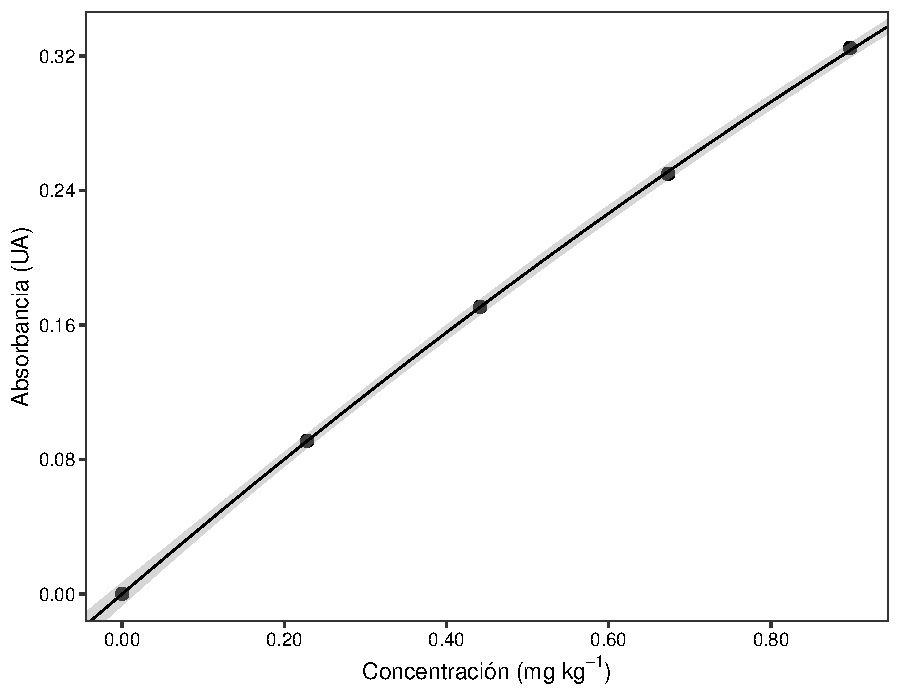
\includegraphics[height=0.388\textwidth]{App/images/MagCalCurves.pdf}}
               \put(24, 168){\large a)}
               \end{picture}}%
    \subbottom{\begin{picture}(230,170)
               \put(0, 0){\includegraphics[height=0.388\textwidth, trim={1.35cm 0 0 0}, clip, page=2]               {App/images/MagCalCurves.pdf}}
               \put(5, 168){\large b)}
               \end{picture}}\\
    \caption[Curvas de calibración para magnesio y calcio por FAAS.]{Curvas de calibración para magnesio (a) y calcio (b) en cloruro de lantano 0.1\% por FAAS. Se incluyen las curvas de regresión donde la zona sombreada gris es el intervalo de confianza para la regresión con una significancia del 99\%.}
    \label{fig:MagCal}
\end{figure}

Las respectivas ecuaciones que describen las curvas de calibración se muestran a continuación:

\begin{equation}
    Abs_{285.2~nm}=(0.000\pm0.001)+(0.412\pm0.005) C_{\ce{Mg^2+}} - (0.057\pm0.004) C_{\ce{Mg^2+}}^2
\end{equation}
\begin{equation}
    Abs_{427.7~nm}=(0.001\pm0.002)+(0.0570\pm0.0005) C_{\ce{Ca^2+}}
\end{equation}
donde la concentración de las especies ($C_{\ce{M^2+}}$) se encuentra en mg~kg\mnn.

\ChapBib{App/App}